\documentclass[]{article}
\usepackage{lmodern}
\usepackage{amssymb,amsmath}
\usepackage{ifxetex,ifluatex}
\usepackage{fixltx2e} % provides \textsubscript
\ifnum 0\ifxetex 1\fi\ifluatex 1\fi=0 % if pdftex
  \usepackage[T1]{fontenc}
  \usepackage[utf8]{inputenc}
\else % if luatex or xelatex
  \ifxetex
    \usepackage{mathspec}
  \else
    \usepackage{fontspec}
  \fi
  \defaultfontfeatures{Ligatures=TeX,Scale=MatchLowercase}
\fi
% use upquote if available, for straight quotes in verbatim environments
\IfFileExists{upquote.sty}{\usepackage{upquote}}{}
% use microtype if available
\IfFileExists{microtype.sty}{%
\usepackage{microtype}
\UseMicrotypeSet[protrusion]{basicmath} % disable protrusion for tt fonts
}{}
\usepackage[margin=1in]{geometry}
\usepackage{hyperref}
\hypersetup{unicode=true,
            pdftitle={Laboratory 1 - Data Driven Security},
            pdfauthor={Arnau Sangrà Rocamora},
            pdfborder={0 0 0},
            breaklinks=true}
\urlstyle{same}  % don't use monospace font for urls
\usepackage{color}
\usepackage{fancyvrb}
\newcommand{\VerbBar}{|}
\newcommand{\VERB}{\Verb[commandchars=\\\{\}]}
\DefineVerbatimEnvironment{Highlighting}{Verbatim}{commandchars=\\\{\}}
% Add ',fontsize=\small' for more characters per line
\usepackage{framed}
\definecolor{shadecolor}{RGB}{248,248,248}
\newenvironment{Shaded}{\begin{snugshade}}{\end{snugshade}}
\newcommand{\KeywordTok}[1]{\textcolor[rgb]{0.13,0.29,0.53}{\textbf{#1}}}
\newcommand{\DataTypeTok}[1]{\textcolor[rgb]{0.13,0.29,0.53}{#1}}
\newcommand{\DecValTok}[1]{\textcolor[rgb]{0.00,0.00,0.81}{#1}}
\newcommand{\BaseNTok}[1]{\textcolor[rgb]{0.00,0.00,0.81}{#1}}
\newcommand{\FloatTok}[1]{\textcolor[rgb]{0.00,0.00,0.81}{#1}}
\newcommand{\ConstantTok}[1]{\textcolor[rgb]{0.00,0.00,0.00}{#1}}
\newcommand{\CharTok}[1]{\textcolor[rgb]{0.31,0.60,0.02}{#1}}
\newcommand{\SpecialCharTok}[1]{\textcolor[rgb]{0.00,0.00,0.00}{#1}}
\newcommand{\StringTok}[1]{\textcolor[rgb]{0.31,0.60,0.02}{#1}}
\newcommand{\VerbatimStringTok}[1]{\textcolor[rgb]{0.31,0.60,0.02}{#1}}
\newcommand{\SpecialStringTok}[1]{\textcolor[rgb]{0.31,0.60,0.02}{#1}}
\newcommand{\ImportTok}[1]{#1}
\newcommand{\CommentTok}[1]{\textcolor[rgb]{0.56,0.35,0.01}{\textit{#1}}}
\newcommand{\DocumentationTok}[1]{\textcolor[rgb]{0.56,0.35,0.01}{\textbf{\textit{#1}}}}
\newcommand{\AnnotationTok}[1]{\textcolor[rgb]{0.56,0.35,0.01}{\textbf{\textit{#1}}}}
\newcommand{\CommentVarTok}[1]{\textcolor[rgb]{0.56,0.35,0.01}{\textbf{\textit{#1}}}}
\newcommand{\OtherTok}[1]{\textcolor[rgb]{0.56,0.35,0.01}{#1}}
\newcommand{\FunctionTok}[1]{\textcolor[rgb]{0.00,0.00,0.00}{#1}}
\newcommand{\VariableTok}[1]{\textcolor[rgb]{0.00,0.00,0.00}{#1}}
\newcommand{\ControlFlowTok}[1]{\textcolor[rgb]{0.13,0.29,0.53}{\textbf{#1}}}
\newcommand{\OperatorTok}[1]{\textcolor[rgb]{0.81,0.36,0.00}{\textbf{#1}}}
\newcommand{\BuiltInTok}[1]{#1}
\newcommand{\ExtensionTok}[1]{#1}
\newcommand{\PreprocessorTok}[1]{\textcolor[rgb]{0.56,0.35,0.01}{\textit{#1}}}
\newcommand{\AttributeTok}[1]{\textcolor[rgb]{0.77,0.63,0.00}{#1}}
\newcommand{\RegionMarkerTok}[1]{#1}
\newcommand{\InformationTok}[1]{\textcolor[rgb]{0.56,0.35,0.01}{\textbf{\textit{#1}}}}
\newcommand{\WarningTok}[1]{\textcolor[rgb]{0.56,0.35,0.01}{\textbf{\textit{#1}}}}
\newcommand{\AlertTok}[1]{\textcolor[rgb]{0.94,0.16,0.16}{#1}}
\newcommand{\ErrorTok}[1]{\textcolor[rgb]{0.64,0.00,0.00}{\textbf{#1}}}
\newcommand{\NormalTok}[1]{#1}
\usepackage{graphicx,grffile}
\makeatletter
\def\maxwidth{\ifdim\Gin@nat@width>\linewidth\linewidth\else\Gin@nat@width\fi}
\def\maxheight{\ifdim\Gin@nat@height>\textheight\textheight\else\Gin@nat@height\fi}
\makeatother
% Scale images if necessary, so that they will not overflow the page
% margins by default, and it is still possible to overwrite the defaults
% using explicit options in \includegraphics[width, height, ...]{}
\setkeys{Gin}{width=\maxwidth,height=\maxheight,keepaspectratio}
\IfFileExists{parskip.sty}{%
\usepackage{parskip}
}{% else
\setlength{\parindent}{0pt}
\setlength{\parskip}{6pt plus 2pt minus 1pt}
}
\setlength{\emergencystretch}{3em}  % prevent overfull lines
\providecommand{\tightlist}{%
  \setlength{\itemsep}{0pt}\setlength{\parskip}{0pt}}
\setcounter{secnumdepth}{0}
% Redefines (sub)paragraphs to behave more like sections
\ifx\paragraph\undefined\else
\let\oldparagraph\paragraph
\renewcommand{\paragraph}[1]{\oldparagraph{#1}\mbox{}}
\fi
\ifx\subparagraph\undefined\else
\let\oldsubparagraph\subparagraph
\renewcommand{\subparagraph}[1]{\oldsubparagraph{#1}\mbox{}}
\fi

%%% Use protect on footnotes to avoid problems with footnotes in titles
\let\rmarkdownfootnote\footnote%
\def\footnote{\protect\rmarkdownfootnote}

%%% Change title format to be more compact
\usepackage{titling}

% Create subtitle command for use in maketitle
\newcommand{\subtitle}[1]{
  \posttitle{
    \begin{center}\large#1\end{center}
    }
}

\setlength{\droptitle}{-2em}
  \title{Laboratory 1 - Data Driven Security}
  \pretitle{\vspace{\droptitle}\centering\huge}
  \posttitle{\par}
  \author{Arnau Sangrà Rocamora}
  \preauthor{\centering\large\emph}
  \postauthor{\par}
  \predate{\centering\large\emph}
  \postdate{\par}
  \date{Spring 2017}


\begin{document}
\maketitle

{
\setcounter{tocdepth}{2}
\tableofcontents
}
\subsection{About the laboratory\ldots{}}\label{about-the-laboratory}

Data Driven Security aims to provide an introduction to computer
security , but from a different perspective.

The goal of the subject is to make you not only aware of the
implications of the analysis of security information data but also
capable to at least explore such data and extract valuable information
in a effective way using the correct methodology.

Throughout the laboratories, the theory seen at class will be put in
practice in conjunction with other tools and technologies related to the
topic. As result, each laboratory will provide you more powerful tools
that usually rely on the previous ones, thus, it is specially important
to complete proposed exercices as well as understand the concepts.

\begin{center}\rule{0.5\linewidth}{\linethickness}\end{center}

~

\section{R Language}\label{r-language}

\begin{center}
\includegraphics[width=150px]{figures/Rlogo} \end{center}

The language used in this subject is \ldots{}\emph{R}. As seen in
theory, there are plenty of reasons to use this programming language for
the tasks where are about to do.

\begin{itemize}
\tightlist
\item
  Ideal for data analysis:

  \begin{itemize}
  \tightlist
  \item
    Powerful
  \item
    Numerous libraries available
  \item
    Easy graphics generation
  \end{itemize}
\item
  Great community of developers
\item
  Open Source
\end{itemize}

\subsection{Hello World!}\label{hello-world}

Following the tradition, the very first program to code with a new
language is the well known \emph{Hello World!}, which shows how to print
a salute.

In R, it would look like this:

\begin{Shaded}
\begin{Highlighting}[]
\KeywordTok{print}\NormalTok{(}\StringTok{"Hello World!"}\NormalTok{)}
\end{Highlighting}
\end{Shaded}

\begin{verbatim}
## [1] "Hello World!"
\end{verbatim}

which unsurprisingly, prints the famous welcoming phrase.

\subsection{Looking for help}\label{looking-for-help}

When progamming, and specially when using a new language, it often
happens that we do not know exactly how to make use of the functions
that implement the feature we are willing to use.

Fortunately, the comunity of R developers usually provides a great
documentation alongside with the package, so that there is a good
description of what does the function do, which parameters accept.

To display the help for a given function, just type a question mark
before the name of the function in the Console:

\begin{Shaded}
\begin{Highlighting}[]
\NormalTok{?help}
\CommentTok{# show help for 'help' function}
\end{Highlighting}
\end{Shaded}

Moreover, documentation usually includes examples with the most common
uses.

\begin{itemize}
\tightlist
\item
  \emph{Look up the documentation for the function print()}
\end{itemize}

\begin{center}\rule{0.5\linewidth}{\linethickness}\end{center}

\section{R Studio}\label{r-studio}

\begin{center}
\includegraphics[width=200px]{figures/RStudio-Logo-Blue-Gradient} \end{center}

Before actually getting our hands dirty writing our R programs to
analyse data, it is a good step to familiarize with the environment we
will be using.

Although it is possible to write R programs in any modern programming
editor, the best environment where to code and execute the R scripts is
undoubtedly \textbf{R Studio}.

This IDE (integrated development environment), available for all major
platforms, including Windows, macOSX and many Linux distributions,
provides a unique framework to develop R programs in a easy but powerful
way. Among the numerous features, RStudio integrates a good source
editor and a R interpreter where to run the code.

Moreover, it also has support for different version control systems like
git and svn, in addition to the set of tools more strictly related to
the R language such as the environment inspector, the package manager or
the plot and the help viewer among others.

\subsection{Configure settings}\label{configure-settings}

Firstly, as a way to know your new IDE, it is very recommendable for you
to inspect the preferences and set them accordingly to your
requirements.

As a good practice and in order to prevent future errors everyone should
agree on a minimal configuration:

\begin{center}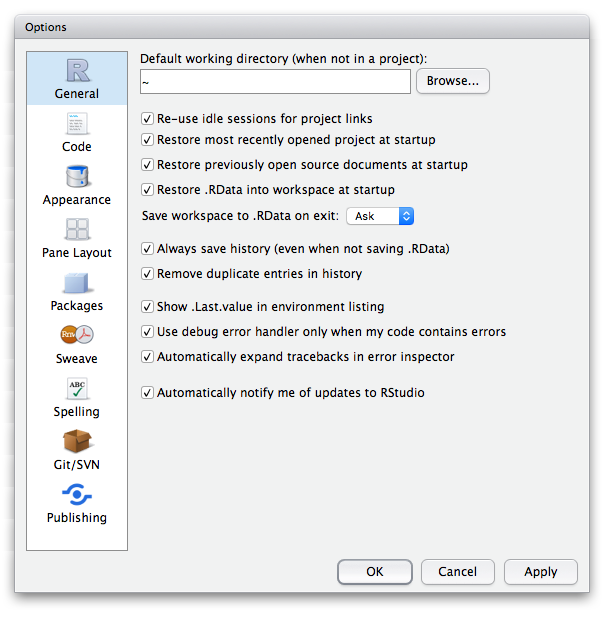
\includegraphics[width=500px]{figures/rstudio_settings} \end{center}

\begin{itemize}
\item
  \emph{Open preferences: (Linux/Windows: Edit -\textgreater{}
  Preferences, OSX: RStudio -\textgreater{} Preferences)}
\item
  Under \emph{Code} section, make sure the following options are checked
  out:

  \begin{itemize}
  \tightlist
  \item
    use \emph{tabs as spaces}, width 2
  \item
    set \emph{soft wrap}
  \item
    set \emph{Strip trailing horizontal whitespace}
  \item
    Saving tab: \emph{Line ending conversion ``Posix (LF)''}
  \item
    Diagnostics tab: \emph{Enable \emph{all} R diagnostics checkboxes}
  \end{itemize}
\item
  Other useful settings:
\item
  Highlight word, currently selected line, R function calls
\item
  show margin (80)
\item
  RMarkdown: -Show output preview in ``Viewer Pane''
\end{itemize}

\subsection{Exploring the layout}\label{exploring-the-layout}

The main RStudio window is divided into 4 different sections that
contain the main different tools that compose the application.

Note that it is possible to customize the layout of the window so that
different sections are arranged differently than default.

\emph{Source} and \emph{Console} sections represent the areas where we
will be spending most of the time. Within \emph{Source} area, we can
view all currently opened files and write our scripts as well.

On the other hand, the console section provides us with an R interpreter
so that we can test our code as much as needed until it works.

\begin{center}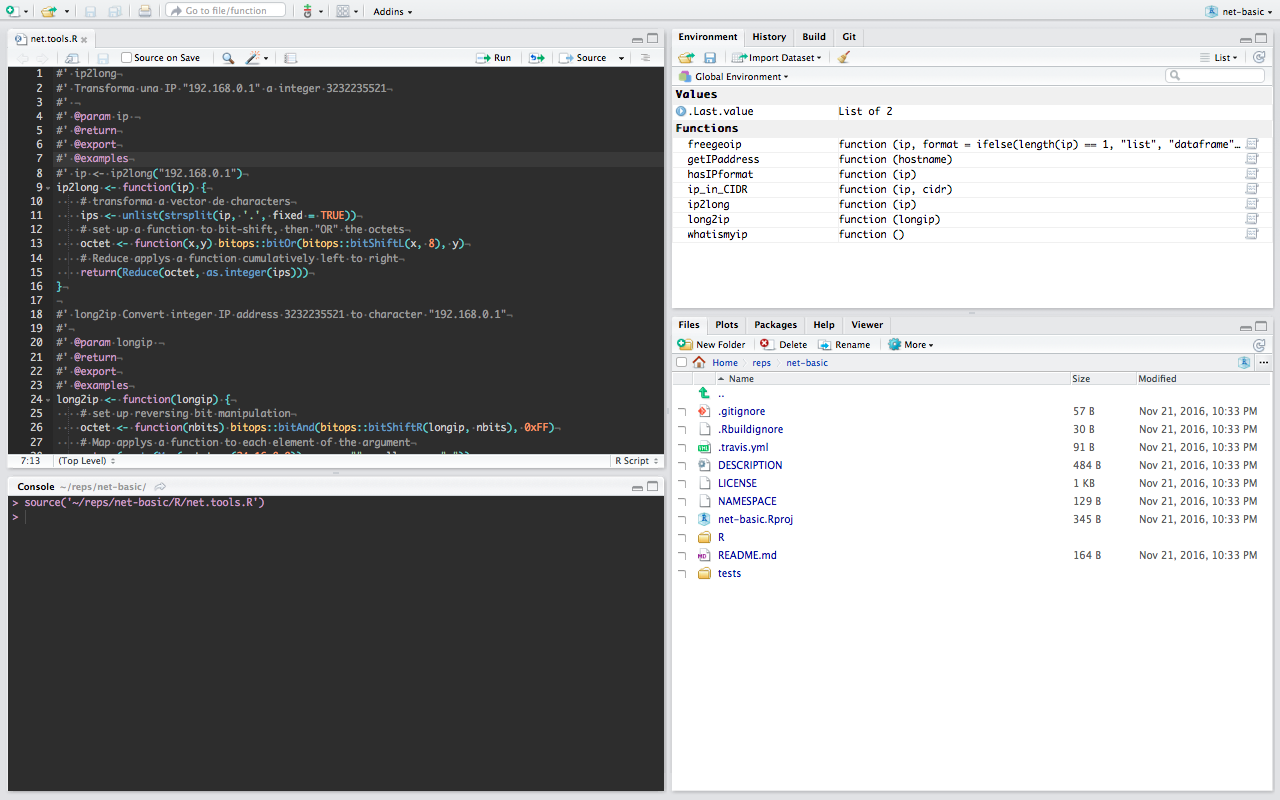
\includegraphics[width=600px]{figures/rstudio_layout} \end{center}

It is not necessary to copy and paste our program's lines from Source to
Console in order to execute. By using \emph{Ctrl + Enter / Cmd + Enter
(macOSX)} we can evaluate the selected line from source and we will
either immediately see the output within the Console or the result of
the execution in the Environment section.

By default, the other two sections grouped beside the Source and the
Console, include the Environment inspector and the history browser in
one pane, and the File Inspector, the package manager and the Plots and
Help Viewer in the other.

\subsection{Debug code}\label{debug-code}

One of the best advantages of using RStudio over other editors is the
possibility to easily debug our programs through its integrated
debugger.

It allows us to set breakpoints to anywhere in our program so that we
can pause the execution at any moment and inspect the environment in
this precise moment.

\begin{itemize}
\tightlist
\item
  \emph{Try setting a breakpoint in any line from the function provided.
  Then execute those and see what happens.}
\end{itemize}

You should see how the console stops at a certain point. At this moment,
the environment section from RStudio should contain all the objects and
their content at the very moment of the execution error. Moreover, you
can also navigate through the stack of environments if any.

\begin{center}\rule{0.5\linewidth}{\linethickness}\end{center}

\section{Git Basics}\label{git-basics}

\begin{center}
\includegraphics[width=200px]{figures/git} \end{center}

\subsection{\texorpdfstring{Create a \emph{hands on} project with R
Studio}{Create a hands on project with R Studio}}\label{create-a-hands-on-project-with-r-studio}

Until now, we have seen a brief introduction to R language and the
RStudio IDE, the editor we will be using to create our programs. Now, it
is time for us to create our first project, that is, the set of files
that will comprise our code, alongside with the configuration settings
and any other thing related to our program.

Since we know a little about \href{https://git-scm.com/}{Git}, the VCS,
we will be using in this course, and is very likely that at some point
we might be interested to share our code, inspect and revert our code to
a functional version and more importantly, to be able work effortlesly
with other people simultaneously, it is a great idea to make our R
project a Git project too.

To do so, just go to File -\textgreater{} New Project, and select the
option ``New Directory'' and ``Empty Project''. Make sure to checkout
the ``create a git repository'' checkbox.

\begin{center}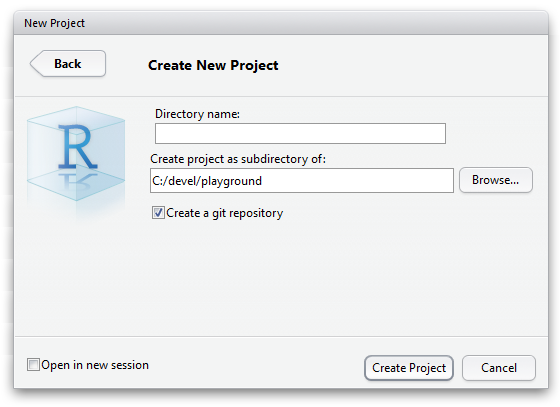
\includegraphics[width=500px]{figures/new_project} \end{center}

That's it. We now have our first R project, the collection of files that
are related to our program.

Notice how a file with \emph{.RProj} extension has been added to the
root of our project folder. It contains the configurations we set for
our project.

Since we have selected the checkbox to create a \emph{git} repository,
RStudio has also initialized our project as a local repository, so that
we can start making changes, adding features and commits and all that
sort of things related to Git.

\begin{itemize}
\tightlist
\item
  \emph{Create a new R file (a normal file with .R extension). Write
  some R code. If you don't have any idea, you can always copy the
  following R program:}
\end{itemize}

\begin{Shaded}
\begin{Highlighting}[]
\CommentTok{# This is my first R program}
\KeywordTok{print}\NormalTok{(}\StringTok{"Hello World!"}\NormalTok{)}

\NormalTok{subject   <-}\StringTok{ "data driven security"}
\NormalTok{language  <-}\StringTok{ "R"}
\KeywordTok{print}\NormalTok{(}\KeywordTok{paste}\NormalTok{(}\StringTok{"This is a hands on project written in"}\NormalTok{,}
\NormalTok{            language,}
            \StringTok{"for "}\NormalTok{,}
\NormalTok{            subject,}
            \StringTok{"subject"}\NormalTok{,}
            \DataTypeTok{sep =} \StringTok{" "}\NormalTok{))}
\end{Highlighting}
\end{Shaded}

\subsection{Commit changes}\label{commit-changes}

Once you have added some R code, you can start by adding all the changes
made to files to the staging area, where it will remain until it is
finally commited.

\begin{center}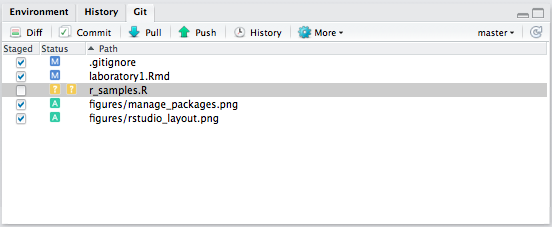
\includegraphics[width=500px]{figures/git_staging} \end{center}

Remember that RStudio provides an easy way to stage the files within the
Git tab, where by default it shows all the files for your project,
allowing you to stage and unstage.

\begin{itemize}
\tightlist
\item
  \emph{Finally, create at least one new commit. Remember to include a
  relevant commmit message regarding the changes included.}
\end{itemize}

\subsection{Create remote repository on
Github}\label{create-remote-repository-on-github}

Although git allows you to work only using a local repository, all the
advantages come with the existance of a remote repository to where to
push the commits hence allowing others to get the changes we make.

To create a remote repository we will be using
\emph{\href{https://github.com/}{GitHub}}, a freemium repository service
on the Internet, where to store our code.

\begin{itemize}
\tightlist
\item
  \emph{Sign up to Github}
\end{itemize}

\begin{center}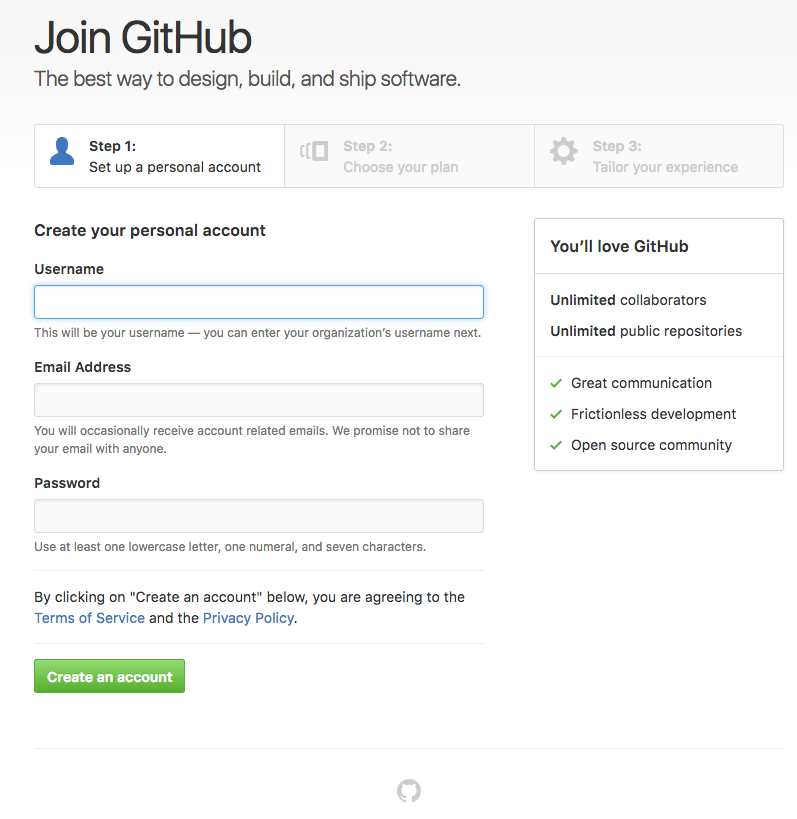
\includegraphics[width=600px]{figures/sign_up_github} \end{center}

\begin{itemize}
\tightlist
\item
  \emph{Create your first repository. To make things easy, name it
  equally to the R project we have just created.}
\end{itemize}

\begin{center}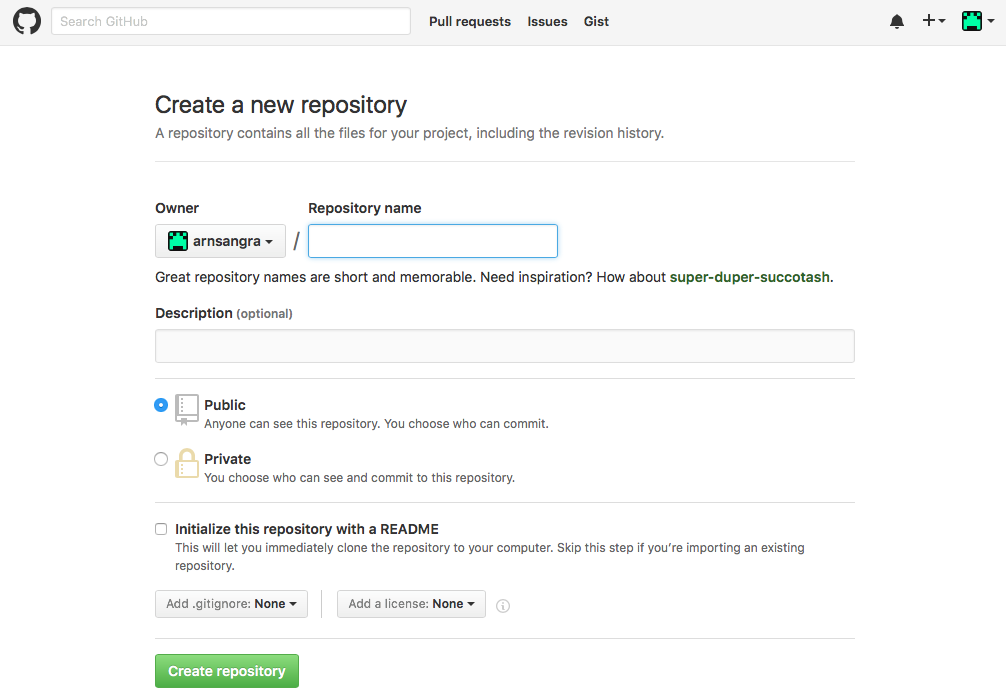
\includegraphics[width=600px]{figures/new_github_repo} \end{center}

Once you have crated the repository, we must somehow establish the
relation between our R project (which is also the local git repository)
and the remote repository before we can actually send our commits to the
Github repository.

\subsection{Link local and remote
repositories}\label{link-local-and-remote-repositories}

In order to share our code, for instance, with any team developer, since
each one will use its own local remote it is necessary to link each
local repository with the central remote (the one provided by GitHub).

In this matter, Despite the existance of other VCS prgrams offer a
graphical interface to easily set the direction of the remote
repository, RStudio still does not provide it unless we initially clone
an R project directly from a remote.

In this particular case, it will be necessary to manually run the git
commands on a shell to establish the remote configuration.

\emph{First of all we must obtain the remote address:}

\begin{center}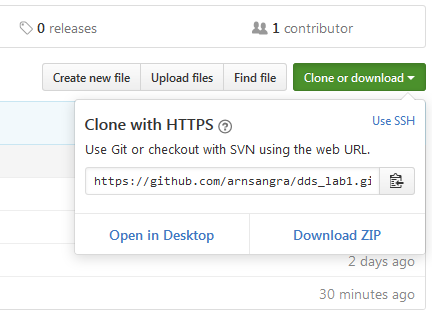
\includegraphics[width=400px]{figures/remote_address} \end{center}

\emph{Then, open a terminal within the project folder and run the git
command to set the direction of the locale}

\begin{Shaded}
\begin{Highlighting}[]
\CommentTok{# substitute '<remote repository address>' with the address copied from GitHub.}
\FunctionTok{git}\NormalTok{ remote add origin }\OperatorTok{<}\NormalTok{remote repository address}\OperatorTok{>}
\end{Highlighting}
\end{Shaded}

If remote address is correct (https or ssh preferably), our local git
repository now is aware of the remote repository.

\subsection{Push to remote}\label{push-to-remote}

Despite the fact of adding the address of the remote, it is still
impossible to share our changes.

Before pushing local commits we must first specify to which branch we
want to send our changes, i.e.~it is still necessary to link the
\emph{local master branch} with the \emph{remote master branch}.

\begin{Shaded}
\begin{Highlighting}[]
\FunctionTok{git}\NormalTok{ push --set-upstream-to=origin/master}
\end{Highlighting}
\end{Shaded}

After issuing the previous command, not only we will have established
the relation between the master branches (local and remote) but also
have send the latest changes made in our local repo to the remote.

\begin{center}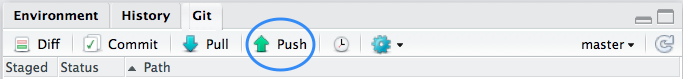
\includegraphics[width=500px]{figures/push_btn} \end{center}

From now onwards, the next time we will want to publish the commits made
from the local repository to the remote, a simple push will be enough.
Since this is a very common action, the green upwards arrow from the git
pane send the new commits to the remote so that other developers can
fetch it.

\subsection{Pull from remote}\label{pull-from-remote}

Lastly, in case we are interested to retrieve the lastest commits pushed
to the team remote repository and integrate this to our code, we can use
the git command pull.

Similarly to the push action, in RStudio, the blue down arrow from the
git pane triggers the pull from the remote.

\begin{center}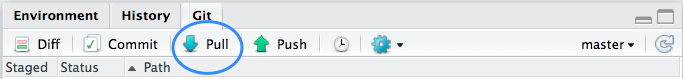
\includegraphics[width=500px]{figures/pull_btn} \end{center}

\begin{center}\rule{0.5\linewidth}{\linethickness}\end{center}

\section{Packages}\label{packages}

Packages play a fundamental role in the development of R applications.
Written by the R community, provide functionalities already implemented
and ready to be used within our programs. Most of the best packages or
libraries are publicly avaiable on
\href{https://cran.r-project.org/}{CRAN} (the Comprehensive R Archive
Network), a very extensive repository for R packages.

However, since CRAN impose certain standards and good practices to
ensure certain minimum quality, packages can also be retrieved from
other source. The other main alternative for R packages is Github. There
we can find not only the those packages that do not satisfy the CRAN
requirements yet, but also the latest bleeding edge versions of most
packages.

\subsection{Manage installed packages with
RStudio}\label{manage-installed-packages-with-rstudio}

To manage installed packages, once again, RStudio provide an easy GUI
interface that facilitates the administration of the packages. Though
it, it is possible to view all already installed packages, install new
ones (from CRAN or local folder), update and uninstall.

\begin{center}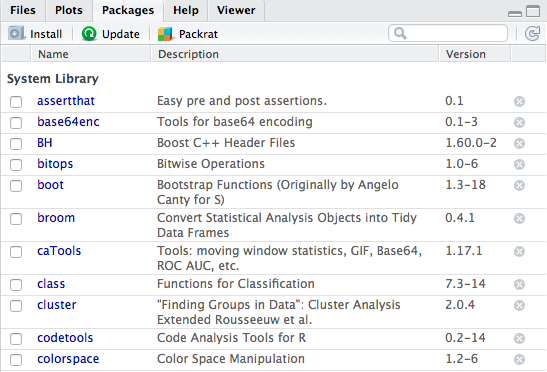
\includegraphics[width=500px]{figures/manage_packages} \end{center}

\begin{itemize}
\tightlist
\item
  \emph{Try installing some of the very useful packages, that are not
  part of the R core:}

  \begin{itemize}
  \tightlist
  \item
    \texttt{xml}
  \item
    \texttt{lubridate}
  \item
    \texttt{stringr}
  \end{itemize}
\end{itemize}

\subsection{Using installed packages}\label{using-installed-packages}

Once a package has been installed, in order to use the functions that
export, i.e.~the features that we want to use, we must firstly load into
memory so that it can be actually used.

To do so, it is as simple as including the installed package within our
program.

\begin{Shaded}
\begin{Highlighting}[]
\KeywordTok{library}\NormalTok{(}\StringTok{"ggplot2"}\NormalTok{)}
\CommentTok{# now we can use functions exported by this package}
\end{Highlighting}
\end{Shaded}

\begin{Shaded}
\begin{Highlighting}[]
\ControlFlowTok{if}\NormalTok{ (}\OperatorTok{!}\KeywordTok{file.exists}\NormalTok{(}\StringTok{"db"}\NormalTok{)) \{}
\NormalTok{  exploitdb_url <-}\StringTok{ "https://github.com/offensive-security/exploit-database/raw/master/files_exploits.csv"}
  \CommentTok{#exploitdb_url <- "https://raw.githubusercontent.com/offensive-security/exploit-database/master/files.csv"}
  \KeywordTok{download.file}\NormalTok{(exploitdb_url, }\DataTypeTok{destfile =} \StringTok{"db"}\NormalTok{)}
\NormalTok{\}}
\NormalTok{db <-}\StringTok{ }\KeywordTok{read.csv}\NormalTok{(}\StringTok{"./db"}\NormalTok{, }\DataTypeTok{header =}\NormalTok{ T)}
\NormalTok{db_aggr <-}\StringTok{ }\NormalTok{dplyr}\OperatorTok{::}\KeywordTok{count}\NormalTok{(db, platform, }\DataTypeTok{sort =}\NormalTok{ T)}
\KeywordTok{ggplot}\NormalTok{(db_aggr, }\KeywordTok{aes}\NormalTok{(}\DataTypeTok{x =} \StringTok{""}\NormalTok{, }\DataTypeTok{y =}\NormalTok{ n, }\DataTypeTok{fill =}\NormalTok{ platform)) }\OperatorTok{+}\StringTok{ }\KeywordTok{geom_bar}\NormalTok{(}\DataTypeTok{width =} \DecValTok{1}\NormalTok{, }\DataTypeTok{stat =} \StringTok{"identity"}\NormalTok{)}
\end{Highlighting}
\end{Shaded}

\begin{center}\includegraphics{laboratory1_files/figure-latex/unnamed-chunk-2-1} \end{center}

This way, we will be able to call the different functions in our code.

For example, using dply and ggplot, we can easily see the top platforms
with more vulnerabilities

\begin{Shaded}
\begin{Highlighting}[]
\NormalTok{db_aggr <-}\StringTok{ }\NormalTok{dplyr}\OperatorTok{::}\KeywordTok{count}\NormalTok{(db, platform, }\DataTypeTok{sort =}\NormalTok{ T)}
\KeywordTok{ggplot}\NormalTok{(}\KeywordTok{head}\NormalTok{(db_aggr), }\KeywordTok{aes}\NormalTok{(}\DataTypeTok{x=}\NormalTok{platform, }\DataTypeTok{y=}\NormalTok{n, }\DataTypeTok{fill=}\NormalTok{platform)) }\OperatorTok{+}\StringTok{ }\KeywordTok{geom_bar}\NormalTok{(}\DataTypeTok{stat =} \StringTok{"identity"}\NormalTok{)}
\end{Highlighting}
\end{Shaded}

\begin{center}\includegraphics{laboratory1_files/figure-latex/unnamed-chunk-3-1} \end{center}

\begin{center}\rule{0.5\linewidth}{\linethickness}\end{center}

\section{Experimenting with the
language}\label{experimenting-with-the-language}

Until now, we have seen the very basics over which we will build up the
future laboratories. In order to familiarize with the R world, it is
necessary to practice a little more.

Since following labs will presuppose certain knowledge of R, you should
complete the swirl introduction, as it represents a great introduction
to the language itself, in a interactive and guided way.

\begin{enumerate}
\def\labelenumi{\arabic{enumi}.}
\tightlist
\item
  \emph{Install Swirl package (either use the packages pane or following
  R instruction on the console):}
\end{enumerate}

\begin{Shaded}
\begin{Highlighting}[]
\ControlFlowTok{if}\NormalTok{ (}\OperatorTok{!}\KeywordTok{require}\NormalTok{(}\StringTok{"swirl"}\NormalTok{)) \{}
  \KeywordTok{install.packages}\NormalTok{(}\StringTok{"swirl"}\NormalTok{, }\DataTypeTok{repos=}\StringTok{"http://cran.rstudio.com/"}\NormalTok{, }\DataTypeTok{quiet =}\NormalTok{ T)}
\NormalTok{\}}
\end{Highlighting}
\end{Shaded}

\begin{enumerate}
\def\labelenumi{\arabic{enumi}.}
\setcounter{enumi}{1}
\tightlist
\item
  \emph{Load the just installed package:}
\end{enumerate}

\begin{Shaded}
\begin{Highlighting}[]
\KeywordTok{library}\NormalTok{(}\StringTok{"swirl"}\NormalTok{)}
\end{Highlighting}
\end{Shaded}

\begin{enumerate}
\def\labelenumi{\arabic{enumi}.}
\setcounter{enumi}{2}
\tightlist
\item
  \emph{Launch swirl and complete the tutorial:}
\end{enumerate}

\begin{Shaded}
\begin{Highlighting}[]
\KeywordTok{swirl}\NormalTok{()}
\end{Highlighting}
\end{Shaded}

\begin{center}\rule{0.5\linewidth}{\linethickness}\end{center}

\section{Complementary references}\label{complementary-references}

\begin{itemize}
\tightlist
\item
  \href{https://www.rstudio.com/wp-content/uploads/2016/01/rstudio-IDE-cheatsheet.pdf}{RStudio
  Cheatsheet}
\item
  \href{http://files.zeroturnaround.com/pdf/zt_git_cheat_sheet.pdf}{Git
  Cheatsheet}
\item
  \href{https://try.github.io/levels/1/challenges/1}{Interactice Git
  Tutorial}
\item
  \href{http://tryr.codeschool.com/}{Interactive R Tutorial}
\item
  \href{https://git-scm.com/book/en/v2}{Git Book}
\end{itemize}


\end{document}
